%%%%%%%%%%%%%%%%%%%%%%%%%%%%%%%%%%%%%%%%%
% Short Sectioned Assignment
% LaTeX Template
% Version 1.0 (5/5/12)
%
% This template has been downloaded from:
% http://www.LaTeXTemplates.com
%
% Original author:
% Frits Wenneker (http://www.howtotex.com)
%
% License:
% CC BY-NC-SA 3.0 (http://creativecommons.org/licenses/by-nc-sa/3.0/)
%
%%%%%%%%%%%%%%%%%%%%%%%%%%%%%%%%%%%%%%%%%

%----------------------------------------------------------------------------------------
%	PACKAGES AND OTHER DOCUMENT CONFIGURATIONS
%----------------------------------------------------------------------------------------

\documentclass[paper=a4, fontsize=11pt]{scrartcl} % A4 paper and 11pt font size
\usepackage[utf8]{inputenc}
\usepackage[MeX]{polski}
\usepackage[T1]{fontenc} % Use 8-bit encoding that has 256 glyphs
\usepackage{fourier} % Use the Adobe Utopia font for the document - comment this line to return to the LaTeX default
 % English language/hyphenation
\usepackage{amsmath,amsfonts,amsthm} % Math packages
\usepackage{graphicx} %images
\usepackage{placeins}%for direct positioning
\usepackage{lipsum} % Used for inserting dummy 'Lorem ipsum' text into the template

\usepackage{sectsty} % Allows customizing section commands
\allsectionsfont{\centering \normalfont\scshape} % Make all sections centered, the default font and small caps

\usepackage{fancyhdr} % Custom headers and footers
\pagestyle{fancyplain} % Makes all pages in the document conform to the custom headers and footers
\fancyhead{} % No page header - if you want one, create it in the same way as the footers below
\fancyfoot[L]{} % Empty left footer
\fancyfoot[C]{} % Empty center footer
\fancyfoot[R]{\thepage} % Page numbering for right footer
\renewcommand{\headrulewidth}{0pt} % Remove header underlines
\renewcommand{\footrulewidth}{0pt} % Remove footer underlines
\setlength{\headheight}{13.6pt} % Customize the height of the header

\numberwithin{equation}{section} % Number equations within sections (i.e. 1.1, 1.2, 2.1, 2.2 instead of 1, 2, 3, 4)
\numberwithin{figure}{section} % Number figures within sections (i.e. 1.1, 1.2, 2.1, 2.2 instead of 1, 2, 3, 4)
\numberwithin{table}{section} % Number tables within sections (i.e. 1.1, 1.2, 2.1, 2.2 instead of 1, 2, 3, 4)

\setlength\parindent{0pt} % Removes all indentation from paragraphs - comment this line for an assignment with lots of text

%----------------------------------------------------------------------------------------
%	TITLE SECTION
%----------------------------------------------------------------------------------------

\newcommand{\horrule}[1]{\rule{\linewidth}{#1}} % Create horizontal rule command with 1 argument of height

\title{	
\normalfont \normalsize 
\textsc{Uniwersytet Wrocławski} \\ [25pt] % Your university, school and/or department name(s)
\horrule{0.5pt} \\[0.4cm] % Thin top horizontal rule
\huge Algorytm Strassena \\
\large Pracownia 1.19 \\ % The assignment title
\horrule{2pt} \\[0.5cm] % Thick bottom horizontal rule
}

\author{Antoni Tomaszewski \\ Artur Derechowski} % Your name

\date{\normalsize\today} % Today's date or a custom date

\begin{document}

\maketitle % Print the title

%----------------------------------------------------------------------------------------
%	PROBLEM 1
%----------------------------------------------------------------------------------------

\section{Opis problemu}

Zadanie polega na napisaniu algorytmu Strassena mnożenia macierzy n*n  i porównania go z klasycznym mnożeniem macierzy. Algorytm Strassena ma złożoność asymptotyczną 
\[ O(N^{\log 7 } )\]
co jest lepsze od standardowego mnożenia w asymptotycznym czasie \[ O(N^{3} )\] Dla dużych macierzy algorytm Strassena powinien więc być szybszy. Algorytm ten zawiera jednak dużą stałą
rzędu $O(N^2)$, dlatego dla małych macierzy spodziewamy się, że będzie on wolniejszy od klasycznego mnożenia.\medbreak
Implementacja algorytmu Strassena została wykonana w języku Julia w pliku "program.jl".
Testy zawierają się w plikach "test.*" i "Wyniki.*".
Wykresy zostały wygenerowane korzystając z biblioteki "Plots".

\section{Algorytm Strassena}

Mając dwie macierze X i Y aby wyznaczyć ich iloczyn można najpierw podzielić je na bloki
\begin{align}
Z = 
\begin{bmatrix}
R & S \\
T & U
\end{bmatrix} &&
X = 
\begin{bmatrix}
A & B \\
C & D
\end{bmatrix} &&
Y = 
\begin{bmatrix}
E & F \\
G & H
\end{bmatrix}
\end{align}
gdzie Z jest iloczynem macierzy X i Y. Następnie trzeba zauważyć, że zamiast robić 8 mnożeń bloków macierzy wystarczy zrobić 7.\\
\begin{align}
R = AE + BH, && S = AG + BH, && T = CE + DF, && U = CG + DH
\end{align}
Tę samą macierz można przedstawić w ten sposób:\\
\begin{align}
R = P5 + P4 - P2 + P6, && S = P1 + P2, && T = P3 + P4, && U = P5 + P1 - P3 - P7
\end{align}
gdzie:\\
\begin{align}
P1 = A(G - H), && P2 = (A + B)H, && P3 = (C + D)E, && P4 = D(F - E), \notag\\
P5 = (A + D)(E + H), && P6 = (B - D)(F + H), && P7 = (A - C)(E + G)
\end{align}

Algorytm Strassena dzieli wtedy macierze na pół i wywołuje na nich kolejne mnożenie Strassena, z analogicznym podziałem dla coraz to mniejszych macierzy. \\

Widać, że algorytm Strassena działa najefektywniej dla macierzy rozmiaru 
${2^k}$. Wtedy zawsze można je dzielić na 2 i wywoływać rekurencyjnie Strassena dla mniejszych macierzy. Gdy macierz jest nieparzystego rozumiaru, to nie można jej pomnożyć, bo nie można jej podzielić na bloki. Problem pojawia się, gdy mamy więc macierz rozmiaru 
${2^k+1}$. Wtedy efektywnie tworzymy macierz 4 razy większą (resztę wypełniamy zerami), aby ją pomnożyć.
W części doświadczalnej pracowni sprawdzamy więc tylko macierze o boku ${2^k}$, aby zilustrować jak najbardziej efektywny algorytm Strassena.
Stała, którą zaniedbujemy nie jest jednak duża, bo w najgorszym przypadku wynosi 4.

\section{Szybkość algorytmu Strassena}

Porównujemy czasy mnożenia dwóch macierzy o danym boku n (tabela 5.1).
Ponieważ algorytm Strassena wyrównuje macierze nie-kwadratowe do macierzy kwadratowych, może tracić na tym dużo czasu.
Dla przykładu pomnożenie wektorów k-elementowych zajmie mu tyle samo czasu, co pomnożenie macierzy kwadratowych o boku k.
Dlatego w pomiarach bierzemy pod uwagę tylko macierze kwadratowe.\medbreak
\begin{table}[h!]
\caption{Czas mnożenie macierzy dwoma sposobami}
\label{my-label}
\begin{tabular}{|l|l|l|l|}
\hline
n	&	Zwykły (wbudowany)	&	Zwykły	&	Strassen (R)	\\  \hline
32	&	2.8482e-5	&	0.000105749	&	0.012895832\\  \hline
64	&	6.0576e-5	&	0.000894503	&	0.089886236\\  \hline
96	&	0.000170009	&	0.003644241	&	0.550218023\\  \hline
128	&	0.000166872	&	0.010069118	&	0.548687255\\  \hline
160	&	0.000330841	&	0.015669477	&	3.860402354\\  \hline
192	&	0.000502141	&	0.022380795	&	3.860977080\\  \hline
224	&	0.000735925	&	0.032780297	&	3.851896002\\  \hline
256 &	0.001038842	&	0.064917801	&	3.846245318\\
\hline
\end{tabular}
\end{table}

Można zauważyć, że algorytm Strassena obecnie wykonuje się o wiele wolniej od wbudowanego operatora mnożenia w języku Julia.
Ten operator może być jednak zaimplementowany o wiele wydajniej, ponieważ jest częścią języka.
Warto w takim razie sprawdzić, jak algorytm Strassena ma się do ręcznie napisanej
funkcji, która działa tak samo jak wbudowany operator, ale nie korzysta z możliwych usprawnień systemowych.\medbreak

Widać, że algorytm Strassena w wersji rekurencyjnej jest również o wiele wolniejszy od napisanej przez nas funkcji mnożącej macierze.
Jest to spowodowane tym, że algorytm tworzy bardzo wiele wywołań rekurencyjnych (aż do macierzy stopnia 1), co znacząco spowalnia czas wykonania programu. \medbreak
Czasy wykonania algorytmu Strassena są natomiast identyczne co do rzędu wielkości dla macierzy o rozmiarach ${\left[2^k, 2^{k+1} \right)}$.
Dzieje się tak, ponieważ w algorytmie Strassena macierze są zawsze wyrównywane do parzystych wielkości poprzez wypełnienie zerami.
Można zauważyć, że wszystkich wyrównań nigdy nie będzie więcej niż czterokrotność całej wielkości macierzy (dla macierzy o boku ${2^k+1}$).
Najefektywniej jest mnożyć macierze o boku ${2^k}$.\medbreak

Dużym problemem w implementacji algorytmu Strassena jest rekurencja.
Implementacja opierająca się na wzorze naturalnie z niej korzysta, jednak dla komputera
jest to proces wolniejszy od iteracyjnego rozwiązania. Rekurencyjna wersja algorytmu 
Strassena jest również o wiele mniej wydajna pod względem pamięciowym, gdzie już dla macierzy niewielkich rozmiarów obserwujemy znaczny wzrost w zaalokowanej pamięci 
(2GB RAM dla macierzy o boku 512 w porównaniu do 2MB dla wersji iteracyjnej).

\section{Efektywny algorytm Strassena}
Naiwna imlementacja algorytmu Strassena nie jest więc wydajna i zachowuje się o wiele gorzej od oczekiwań.
Jest to spowodowane dużym kosztem wielu wywołań rekurencyjnych dla małych macierzy, które możnaby szybko policzyć mnożący klasycznie.
Skoro dla małych macierzy nie opłaca się mnożyć algorytmem Strassena,
to implementację algorytmu Strassena będziemy zatrzymywać na pewnej stałej, którą wyznaczamy eksperymentalnie.
Do pewnego momentu dzielimy duże macierze algorytmem Strassena.
Gdy natomiast bok macierzy jest mniejszy od pewnej stałej, macierze są mnożone klasycznie.\medbreak

\begin{figure}[h!]
  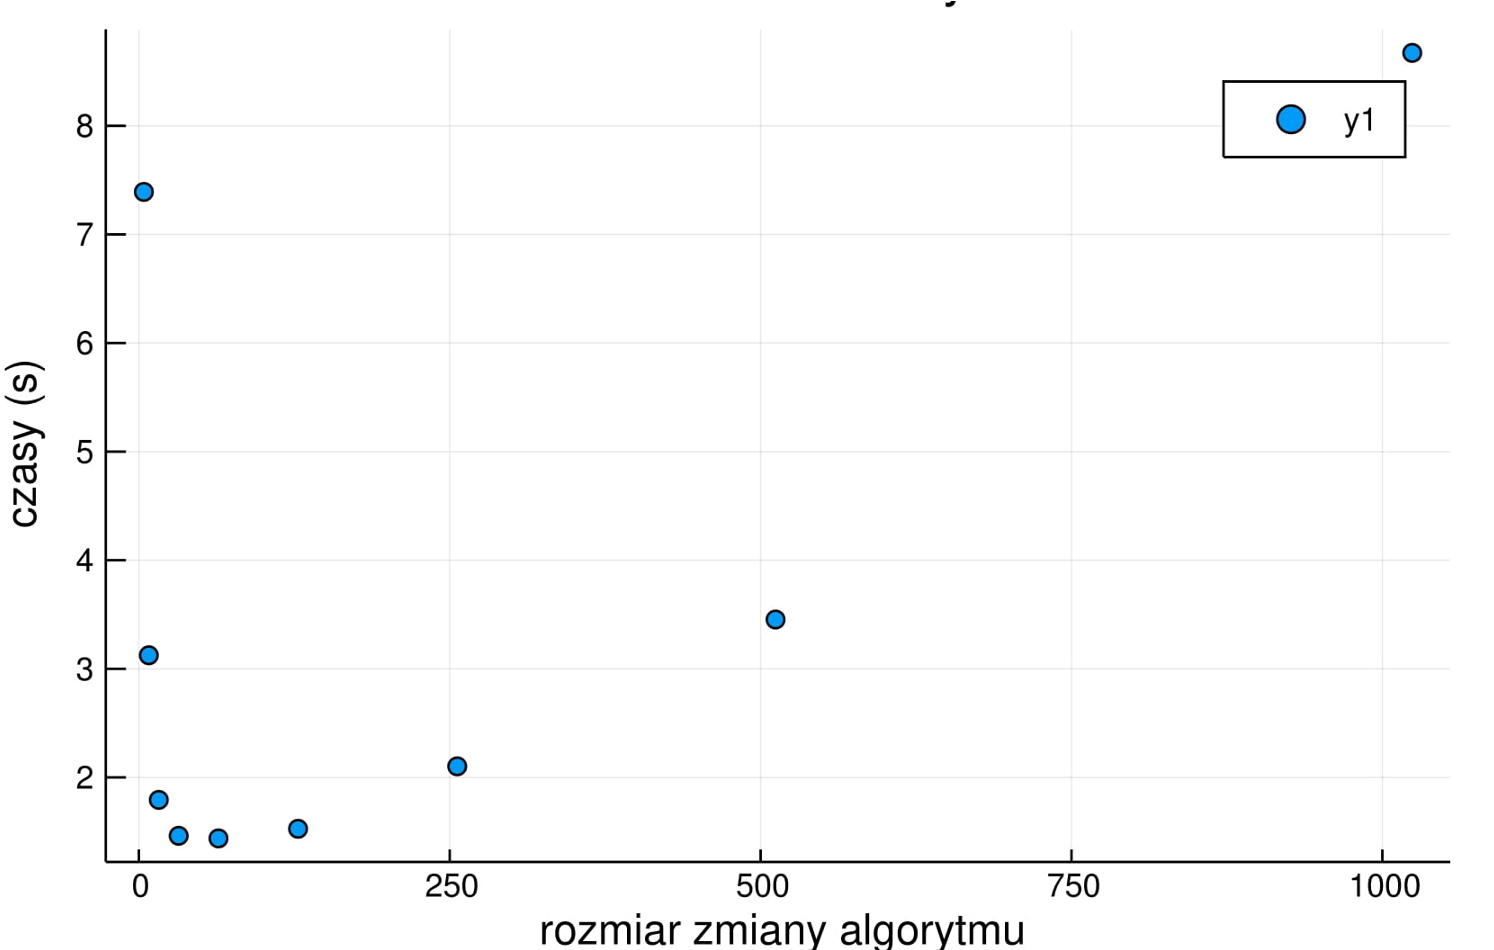
\includegraphics[width=0.95\linewidth]{krok.jpg}
  \caption{Czas mnożenia dla macierzy 1024x1024 z różnymi punktami przejścia}
  \label{szybkosc}
\end{figure}
\begin{figure}[h!]
  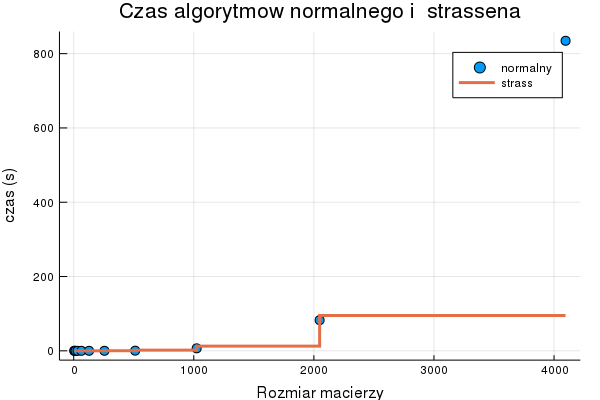
\includegraphics[width=0.95\linewidth]{szybkosc.png}
  \caption{Czas lepszego mnożenia macierzy Strassena i klasycznego mnożenia}
  \label{szybkosc}
\end{figure}
 
Dzięki temu uzyskujemy algorytm, który wykorzystuje lepszą złożoność algorytmu Strassena, 
jednocześnie nie traci jednak na dużej ilości mnożeń małych macierzy, które musi wykonać.\medbreak

Do wyznaczenia najlepszego punktu przejścia algorytmu sprawdzamy wszystkie możliwe wartości postaci ${2^n}$.
Widać, że minimum osiągane jest przy wartości 64, na wykresie \ref{krok}.\medbreak
Wykorzystując ten algorytm, uzyskujemy już wyniki, które są istotnie szybsze dla macierzy dużych rozmiarów. \ref{szybkosc}
\FloatBarrier


\section{Analiza błędów}
Ważnym wskaźnikiem jakości algorytmu jest nie tylko jego szybkość, ale także jak bardzo dokładny jest numerycznie.
Przeprowadzamy obliczenia dla macierzy o rozmiarach od 4 do 1024, 
sprawdzając każdą potęgę dwójki (wtedy algorytm Strassena jest różny względem każdej iteracji). Dla danej macierzy nieosobliwej liczymy wartości błędów 
$\Delta(X X^{-1} - I)$ oraz $\Delta(X^{-1}X - I)$ , gdzie 
$${\Delta(X) := \sum_{i=1}^n \sum_{j=1}^n x_{i,j}^2 }$$ \medbreak

Na wykresie \ref{blad} widać, że błędy obliczeń w algorytmie Strassena tylko nieznacznie różnią się od błędów w klasycznym mnożeniu.
Większą różnicę ma natomiast kolejność wykonywania mnożenia.
Lepszą dokładność obserwujemy, mnożąc ${A A^{-1} }$ niż ${A A^{-1} }$.\medbreak

Następnie porównujemy algorytm Strassena pod względem dokładności mnożąc macierze ${(X Y)Z - X(Y Z) }$ coraz to większych rozmiarów.
Mnożenie macierzy jest łączne, więc uzyskany błąd powinien być jak najmniejszy. 
Na wykresie \ref{xyz} widać jednak, że w tym przypadku algorytm Strassena daje mniejszą dokładność od klasycznego mnożenia.

\begin{figure}[h!]
  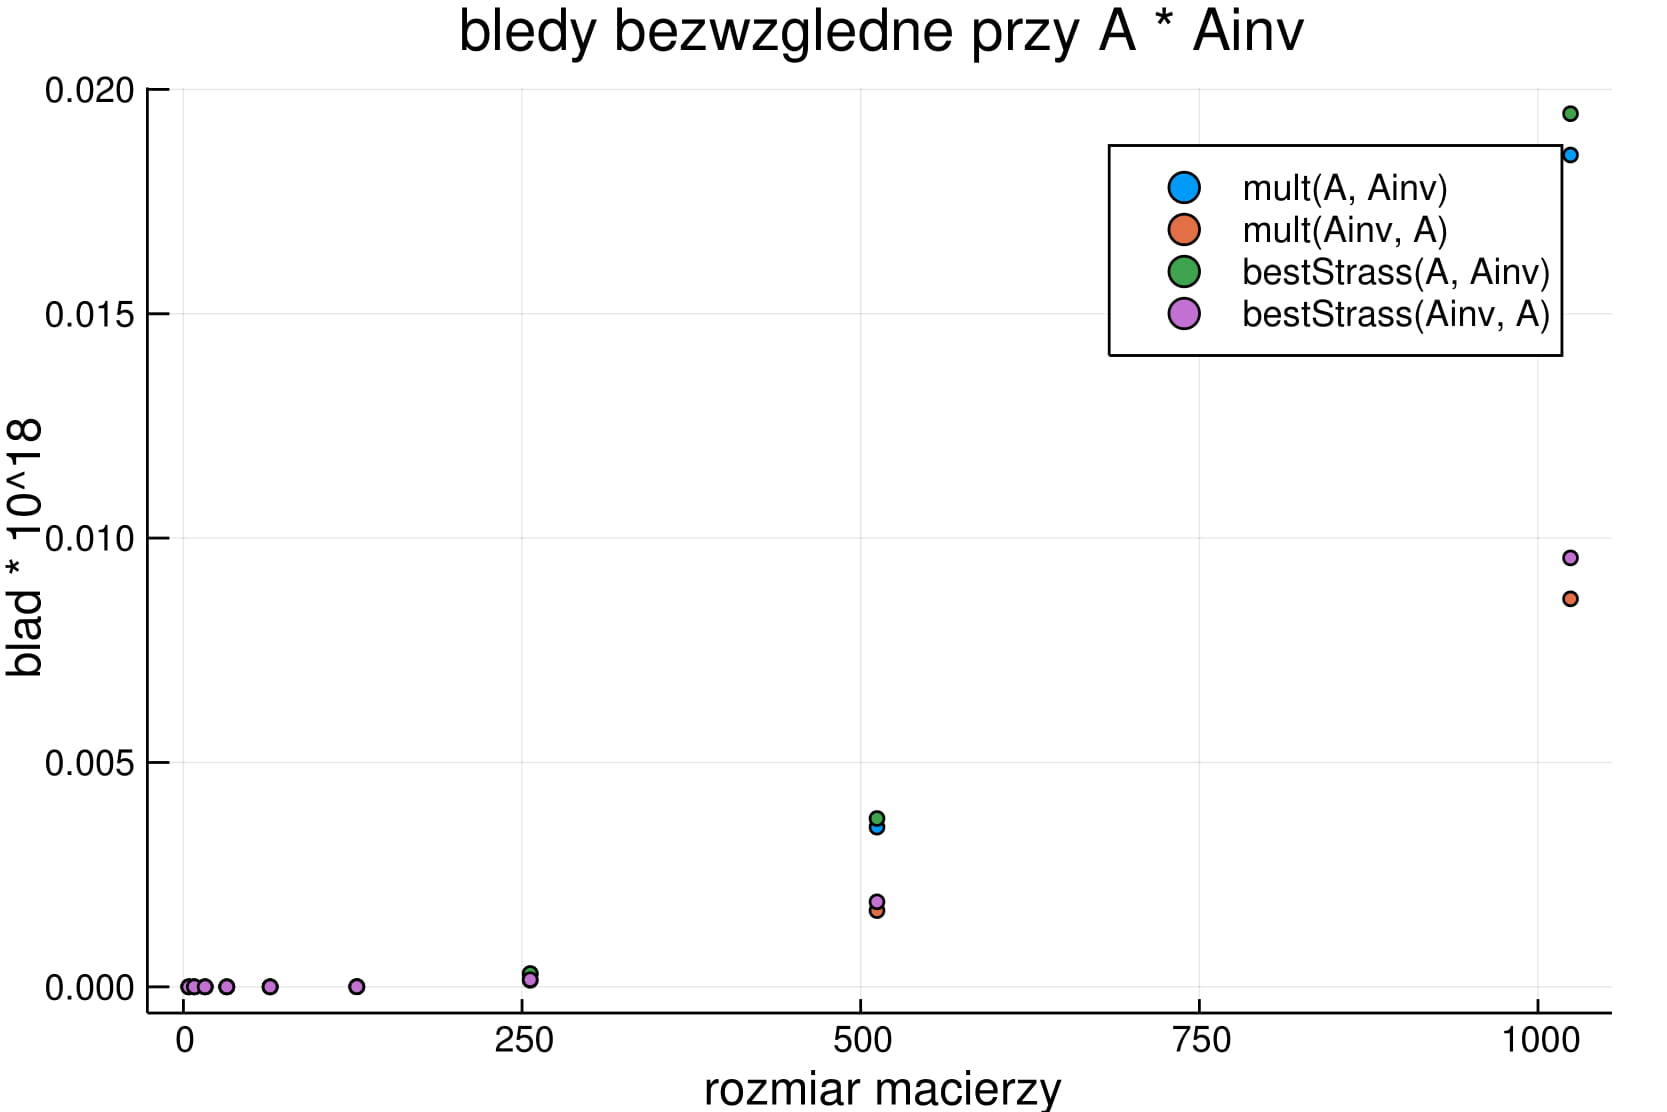
\includegraphics[width=\linewidth]{inv.jpg}
  \caption{Błędy $\Delta(A^{-1}A - I)$ i $\Delta(A A^{-1} - I)$ algorytmu Strassena}
  \label{blad}
\end{figure}

\begin{figure}[h!]
  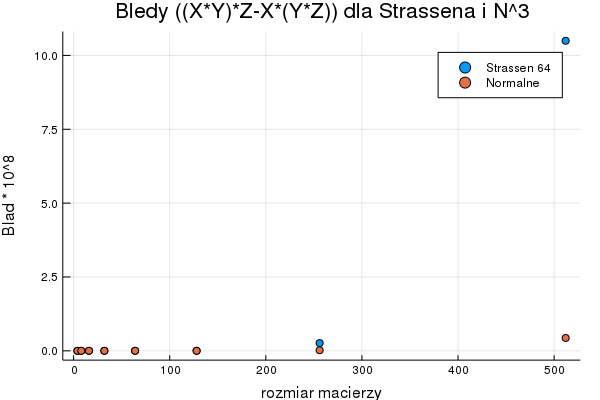
\includegraphics[width=\linewidth]{BladXYZ.png}
  \caption{Błędy $\Delta(A^{-1}A - I)$ i $\Delta(A A^{-1} - I)$ algorytmu Strassena}
  \label{xyz}
\end{figure}

% w tabeli wystarczy iść tak co 4 plus wszystkie postaci (2^k )-1, czyli byłaoby z 50 pomiarów
% ogólnie to te tabele najłatwiej robić używając tej stronki: http://www.tablesgenerator.com/  
% Jak będziemy mieli wyniki to wystarczy je zapisać w pliku .csv i można go załadować

\FloatBarrier

\section{Mnożenie kwaternionów}
Algorytm Strassena daje oszczędność jednego mnożenia na osiem. Istnieją jednak inne przekształcenia,
które mogą bardziej zmniejszyć liczbę kosztownych mnożeń na rzecz dodawania. Przykładem tego jest mnożenie kwaternionów.

\subsection{Kwaterniony}
Kwaternion jest strukturą algebraiczną rozszerzającą liczby zespolone:
\[q = a + bi + cj + dk \]
gdzie ${a,b,c,d}$ są liczbami rzeczywistymi,
 \[i^{2}=j^{2}=k^{2}=ijk=-1 \]
Mnożąc klasycznie dwa kwaterniony zgodnie z zasadą rozdzielności wykonamy 16 mnożeń:\medbreak
\begin{equation}
	\begin{gathered}
	(x_1 + x_2 i + x_3 j + x_4 k ) * (y_1 + y_2 i + y_3 j + y_4 k) = f1 + f2 + f3 + f4 \\
	f_1 = x_1 y_1 - x_2 y_2 - x_3 y_3 - x_4 y_4 \\
	f_2 = (x_1 y_2 + x_2 y_1 + x_3 y_4 - x_4 y_3 ) i \\
	f_3 = ( x_1 y_3 - x_2 y_4 + x_3 y_1 + x_4 y_2 ) j \\
	f_4 = ( x_1 y_4 + x_2 y_3 - x_3 y_2 + x_4 y_1 ) k	
	\end{gathered}
\end{equation}

\subsection{Przekształcenie}
Zapiszemy powyższą sumę w inny sposób, wykonując tylko 8 mnożeń zamiast 16. Niech:
\begin{equation}
\begin{gathered}
\\
[I] = x1 y1 \\ 
[II] = x4 y3 \\ 
[III] = x2 y4 \\
[IV] = x3 y2 \\
[V] = (x1+x2+x3+x4)(y1+y2+y3+y4) \\
[VI] = (x1+x2-x3-x4)(y1+y2-y3-y4) \\
[VII] = (x1-x2+x3-x4)(y1-y2+y3-y4) \\
[VIII] = (x1-x2-x3+x4)(y1-y2-y3+y4) \\
\end{gathered}
\end{equation}

Wtedy sumę ${f_1+f_2+f_3+f_4}$ można zapisać jako:

\begin{equation}
\begin{gathered}
\\
f_1 = 2[I] - ([V] + [VI] + [VII] + [VIII])/4 \\ 
f_2 = -2[II] + ([V] + [VI] - [VII] - [VIII])/4 \\ 
f_3 = -2[III] + ([V] - [VI] + [VII] - [VIII])/4 \\
f_4 = -2[IV] + ([V] - [VI] - [VII] + [VIII])/4 \\
\end{gathered}
\end{equation}

Widać więc, że iloczyn dwóch kwaternionów można wykonać, robiąc tylko 8 mnożeń zamiast 16\cite{quaternion}. 
Zapisanie tego przekształcenia w innej postaci pozwala więc na poprawę liczby mnożeń o ${50\%}$., 
podczas gdy algorytm Strassena mnożenia macierzy pozwalał jedynie na ${12,5\%}$ oszczędności.\medbreak
Dla algorytmu mnożącego kwaterniony można udowodnić, że nie da się go wykonać z liczbą mnożeń mniejszą niż 8.\cite{quaternion}

\section{Wnioski}
Algorytm Strassena, który daje lepszą złożoność obliczeniową, może być wykorzystany
tylko do mnożenia określonych macierzy 
(kwadratowych, o dużym rozmiarze, o których wiemy, że nie zawierają dużej ilości zer).
W takim przypadku jest on jednak kilkukrotnie szybszy, co może mieć znaczenie w praktyce.
Z powodu ograniczeń sprzętowych (pamięć RAM) największe macierze jakie testowaliśmy
to 1024 na 1024.
Po obejściu tego problemu można jednak mnożyć macierze dwukrotnie lub czterokrotnie większe, 
dla których różnica pomiędzy czasem mnożenia Strassena a klasycznym będzie o wiele bardziej widoczna.

\begin{thebibliography}{9}

\bibitem{quaternion}
  Thomas D. Howell,
  Jean-Cleaude Lafon,
  \textit{The Complexity of the Quaternion Product}, \\
  Department of Computer Science, Cornell University, Ithaca, N.Y.
  1975.

\bibitem{strassen}
  Volker Strassen,
  \textit{Gaussian Elimination is not Optimal}, \\
  Numerische Mathematik 13, p. 354-356, 1969
\end{thebibliography}

\end{document}
